\chapter{Planned Implementation}
\section{Emotion Input}
This will be an interface, that end users use for inputting emotions. It will consist of a slider for each emotion for that particular media(i.e. separate emotions for movies and songs). The value will be a floating point number with a range from 0 to 1. Once the emotions are submitted by the end user, they will be normalized by dividing each emotion by the sum of all emotions. i.e.

 $$ E_{a} = \frac{e_{a}}{\sum_{i=0}^{n}{e_{i}}} $$
\begin{align*}
\text{where } E_{a} &= \text{Normalized value of } e_{a}  \\
e_{i} &= \text{magnitude of emotion } e_{i} \text{ as input by user}\\
n &= \text{number of emotions accepted}
\end{align*}

\section{Authentication}
To be implemented with Auth0, JSON Web Tokens (JWTs) and the modern OAuth 2.0 framework. We will be providing login using various services like Google, Twitter, GitHub etc. This increases security by avoiding the need to have the user remember a secure and complicated password. The aim is to make the authentication process as simple as ‘one click to get started’. This approach also allows us to reuse industry standard components rather than needing to reinvent the wheel. The architecture of OAuth 2.0 is shown in Figure \ref{fig: oAuth uml}

\begin{figure}[H]
\centering
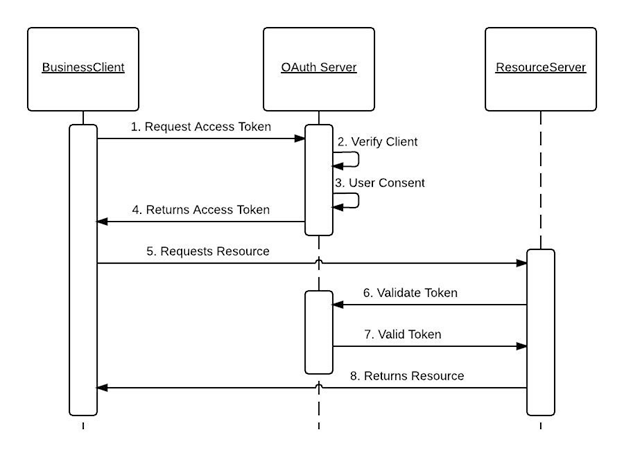
\includegraphics[width=\textwidth]{imgs/oAuth.png}
\caption{OAuth 2.0 Architecture Diagram}
\label{fig: oAuth uml}
\end{figure}
\section{Song Classifier}

\subsection{The Dataset}
2 datasets will be used to train the model, namely:
\begin{enumerate}
	\item The GTZAN dataset
	\item A custom dataset of around 200 songs hand labeled 
\end{enumerate}
The custom dataset will be generated by us using a data collection tool as detailed below.

\subsection{The Model}
The initial architecture of the model to be trained is based on a paper by Ceylan et. al. \cite{ceylan_automatic_2021}. It involves using Mel Frequency Cepstrums(MFC’s) as inputs to a CNN. MFC’s allow us to visualise the different features of a signal at different points of time. \newline

The model will be trained on genre detection using the GTZAN dataset. Once sufficient accuracy is achieved, transfer learning will be used to train the model on the custom dataset to obtain the output we desire. \newline


Two kinds of models will be investigated, namely

\begin{enumerate}
	\item Artificial neural network (ANN)
	\item Convolution neural network (CNN)
\end{enumerate}
The ANN will consist of only dense layers and will take tabular inputs. These inputs will be descriptive features of the input songs like MFCC, spectral centroid, spectral rolloff, chroma frequencies, tempo etc. The CNN will take MFC visualizations and spectrograms as inputs.

\subsection{Model Architecture}

\begin{figure}[H]
\centering
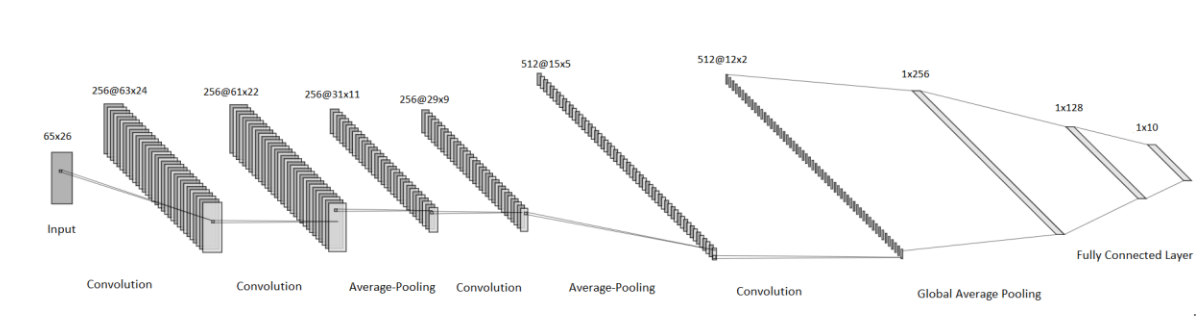
\includegraphics[width=\textwidth]{imgs/model_architecture.png}
\caption{CNN Model Architecture}
\label{fig: cnn architecture}
\end{figure}


The model used in the paper has the following architecture as shown in Figure \ref{fig: cnn architecture}:

\begin{itemize}
	\item Convolution Layer with filters: 256, kernel size: 3x3, 
	\item Convolution Layer with filters: 256, kernel size: 3x3, 
	\item Average Pooling with pool size: 3x3, strides: 2x2, 
	\item Convolution Layer with filters: 256, kernel size: 3x3,
	\item Average Pooling with pool size: 3x3, strides: 2x2, 
	\item Convolution Layer with filters: 512, kernel size: 4x4, 
	\item Global Average Pooling,
	\item Fully Connected Layer,
	\item Dense Layer with units: 256, 
	\item Dense Layer with units: 128, 
	\item Dense Layer with units: 10, activation function: softmax
\end{itemize}

\section{Movie Classifier}
\subsection{The Dataset}
The dataset that will be used to train the model is the XED dataset. This dataset maps movie subtitles to Plutchik's wheel of emotions. Each record in this dataset is an individual sentence mapped to an emotion. \newline

\subsection{The Model}
The model will be a RNN, i.e. it will have one or more recurrent layers like a LSTM or GRU layer. This model will be trained on individual lines from subtitles. To classify a movie, the model will be run on every line of its subtitles. Lines that get classified as neutral are discarded. The sum of the number of lines belonging to each emotion category are then normalized. This gives us a single vector of emotions with values ranging from 0 to 1.
\subsection{Model Architecture}
The initial architecture of the model to be trained will be based on a paper by Hidayatullah et. al. \cite{rnn-sentiment}, where sentiment analysis was used on twitter data to predict the winner of the Indonesian Presidential Election. The model architecture used in the paper is shown in Figure \ref{fig: movieModelArch}


\begin{figure}[H]
\centering
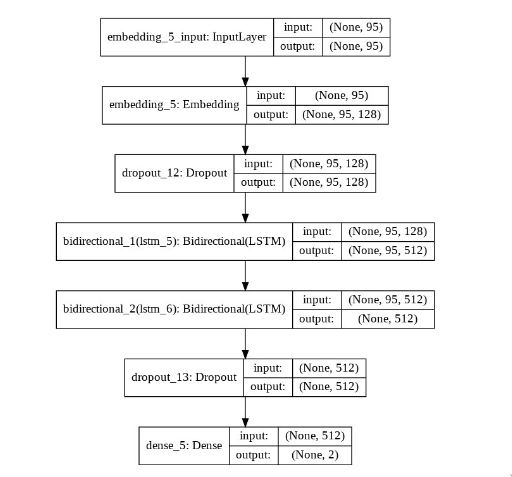
\includegraphics[width=\textwidth]{imgs/movieModelArch.png}
\caption{Sentiment Analysis Model Architecture}
\label{fig: movieModelArch}
\end{figure}
The main change to be made to this model for the purposes of this project is to change the number of neurons in the final layer to the number of emotions we want to predict. 
\section{Media Search \& Recommender System:}
This system will consist of 2 modules i.e. a Media Lookup Module and a Recommender System.

\begin{figure}[H]
\centering
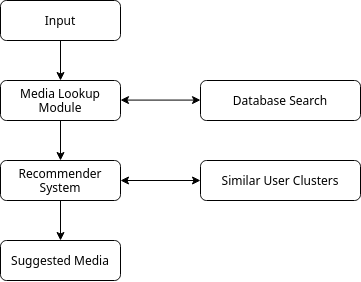
\includegraphics[scale=0.6]{imgs/mediaSearchuml.png}
\caption{Flow for Media Search and Recommender Module}

\label{fig: mediaUML}
\end{figure}
\subsection{Media lookup module}
Based on the user’s inputted emotions, this module will perform a search on the classified songs and movies in the database and return the closest 20 items. To find the best matches, distance measures based on Minkowski distance like Euclidean and Manhattan distance, and also Cosine distance will be tested. The distance measure with the best results will be picked.

\subsection{Recommender System}
Since emotions are subjective, if one movie in the database is slightly closer to the inputted emotion than another movie, it doesn't necessarily mean that the closer movie is better. To address this subjectivity in the inputted emotion, the Media Search module is augmented by a recommendation system that users similar users preferences to decide which movies/songs should be ranked higher, i.e. which movies/songs are better matches for that particular user. \newline

As the user views the songs/movies, if he/she rates them, that rating is stored and used for future recommendations. Once the user has some minimum threshold number of ratings, we can augment the simple search with a recommendation system.

\subsubsection{Prerequisites}
\begin{enumerate}
	\item A matrix of user-movie ratings as shown in Figure \ref{fig: user movie ratings} will be maintained
	\item Users should periodically be clustered based on their movie ratings using KNN algorithm
\end{enumerate}

\begin{figure}[H]
\centering
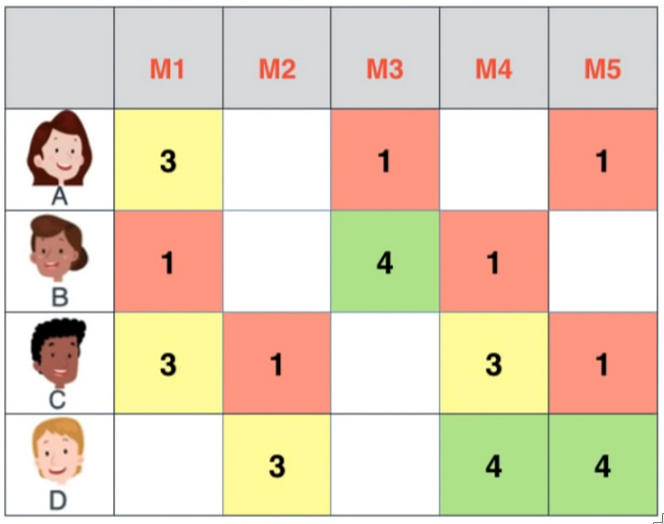
\includegraphics[scale=0.5]{imgs/user-movie ratings.png}
\caption{User-Movie ratings matrix}
\label{fig: user movie ratings}
\end{figure}

\subsubsection{Recommendation Algorithm}
To recommend new movies to a particular user A:
\begin{enumerate}
	\item Consider the ratings of all other users in the same cluster
	\item Take a weighted average of all movies user A hasn’t seen. Let the weight be the inverse of distance of that user from user A
	\item Recommend the movies with highest score to user A
\end{enumerate}

To illustrate we have also included the formula here below :
$$ Score = \frac{\sum_{i=0}^{m}{\frac{R_{i}}{d_{i}}}}{n}      $$

\begin{align*}
\text{where } R_{i} &= \text{Ratings by user} i  \\
d_{i} &= \text{distance between user } A \text{and user }i\\
n &= \text{number of users in cluster} \\
m &= \text{number of movies in matrix}
\end{align*}

\section{Data Collection Tool}
The capabilities of this tool is as follows:
\begin{itemize}
	\item A tool that connects to Spotify and allows the user to search for and label songs.
	\item Search for a song, listen to it and label it from just one location.
	\item Designed for mobile usage as well, so it can be used on the go too.
\end{itemize}

This tool is built into our application as an admin dashboard. It utilizes Spotify’s API which is free for non-commercial usage to fetch song data. It is connected to MongoDB via Node.js APIs.
\subsection{Desktop View}
\begin{figure}[H]
\centering
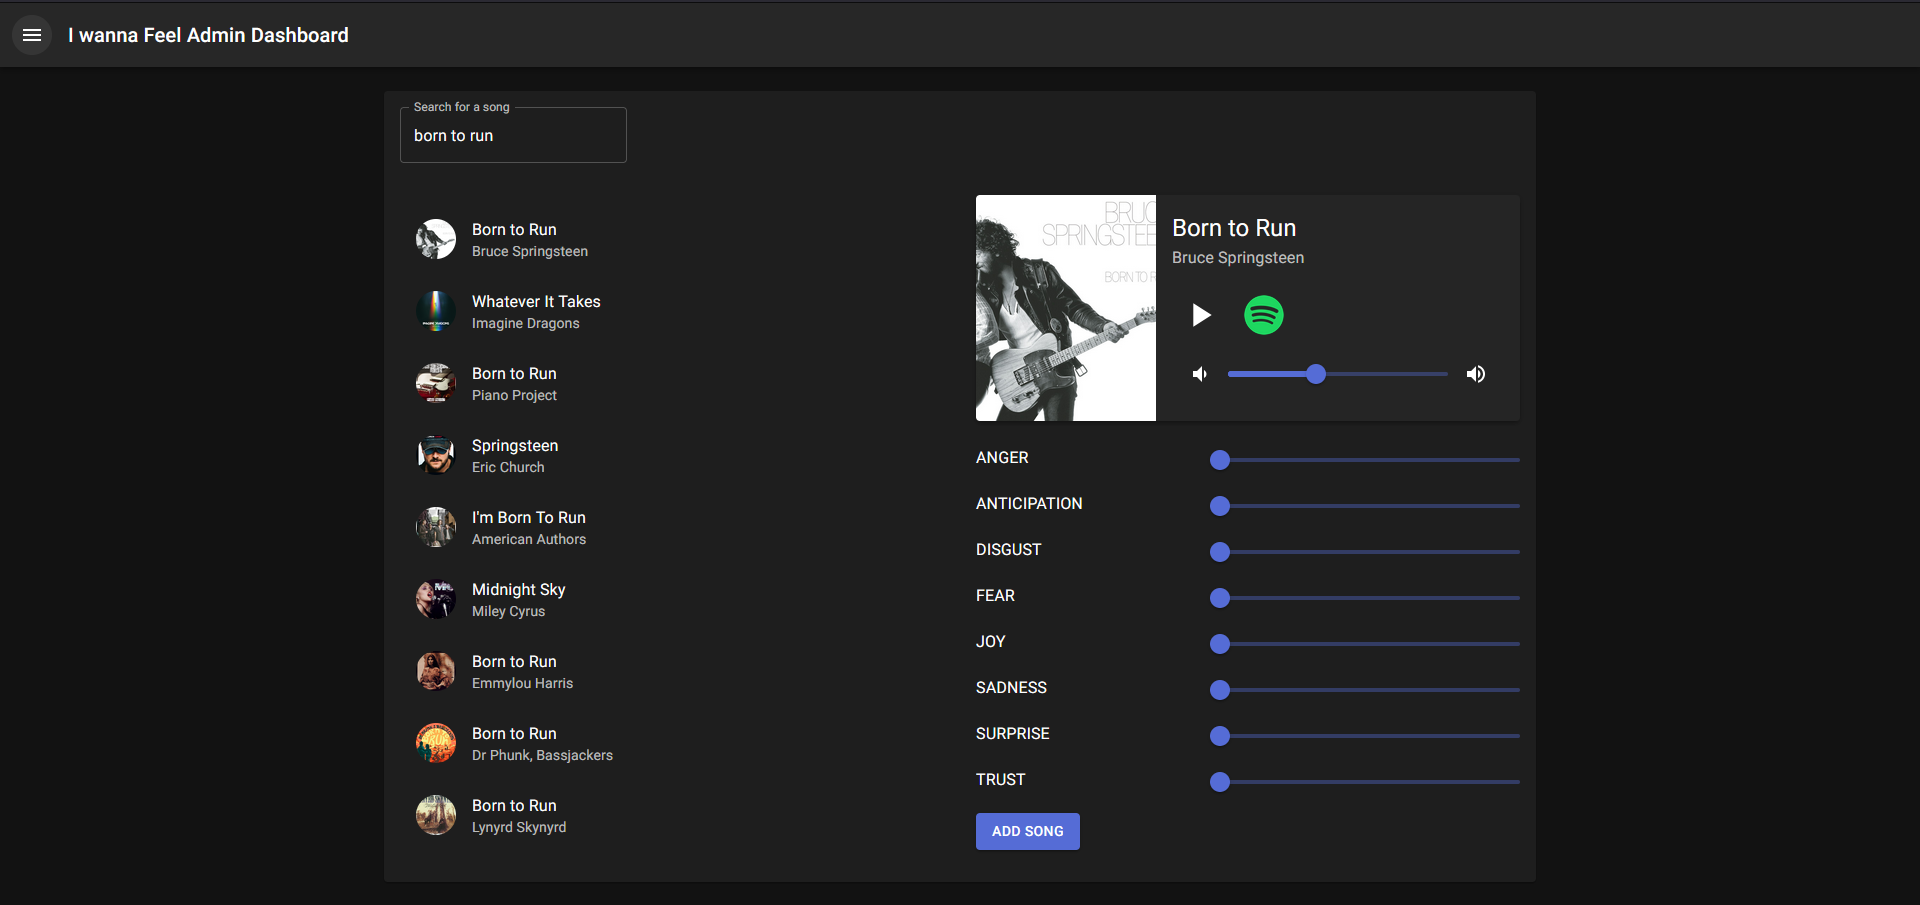
\includegraphics[width=\textwidth]{imgs/data_collection_1.png}
\caption{Section to search, play and label songs}
\label{fig: data_collection_1}
\end{figure}

\begin{figure}[H]
\centering
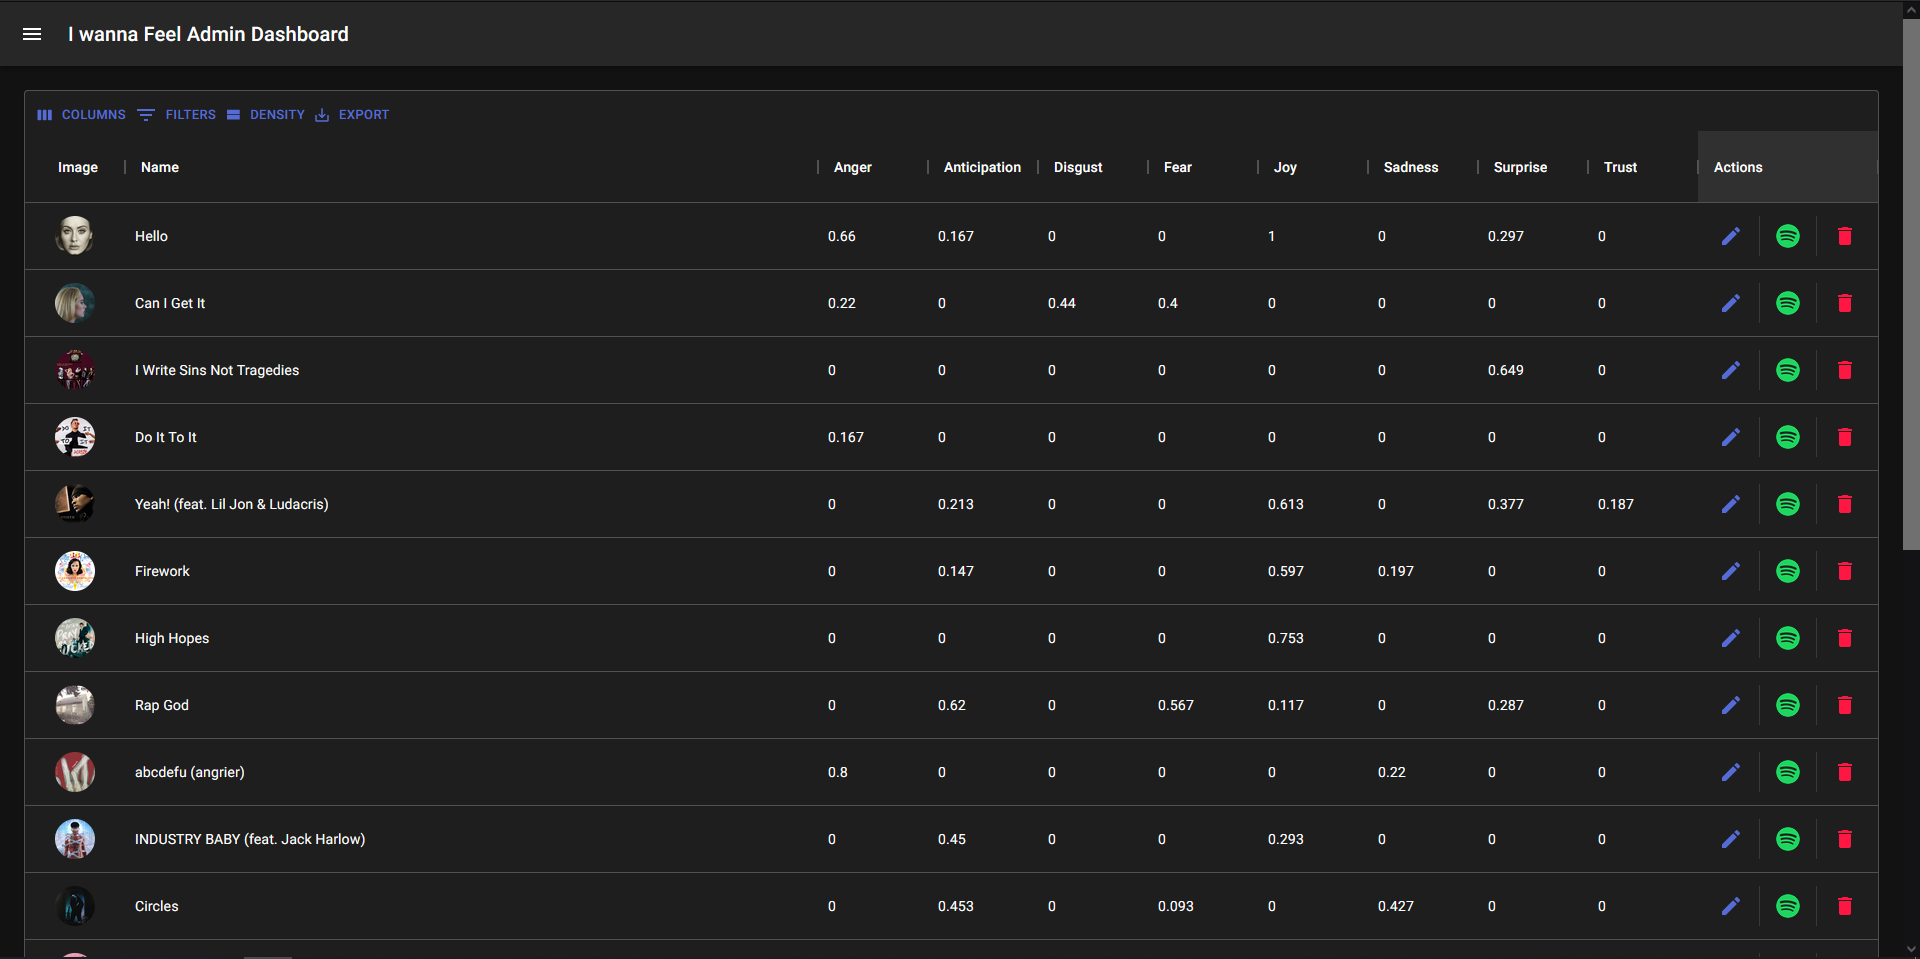
\includegraphics[width=\textwidth]{imgs/data_collection_2.png}
\caption{Section to search, filter, update, delete songs}
\label{fig: data_collection_2}
\end{figure}

\subsection{Mobile View}

\begin{figure}[H]
\centering
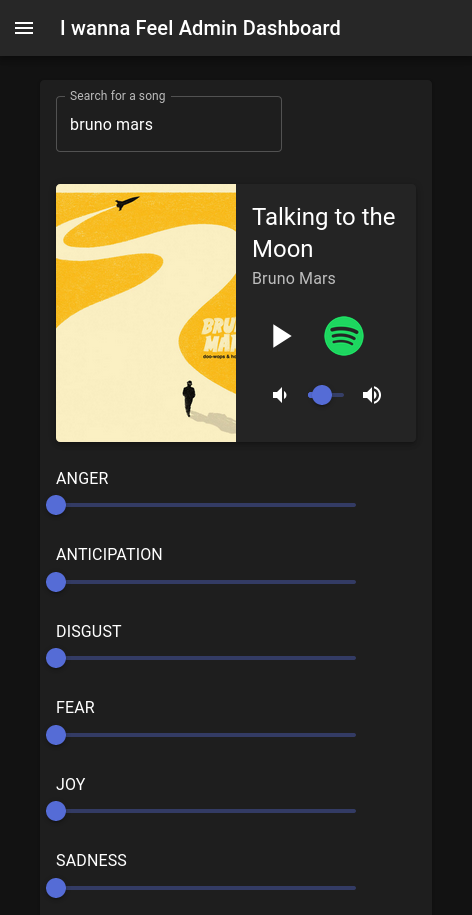
\includegraphics[scale=0.6]{imgs/mobileui1.png}
\caption{Emotion input}
\label{fig: mobileUI_1}
\end{figure}

\begin{figure}[H]
\centering
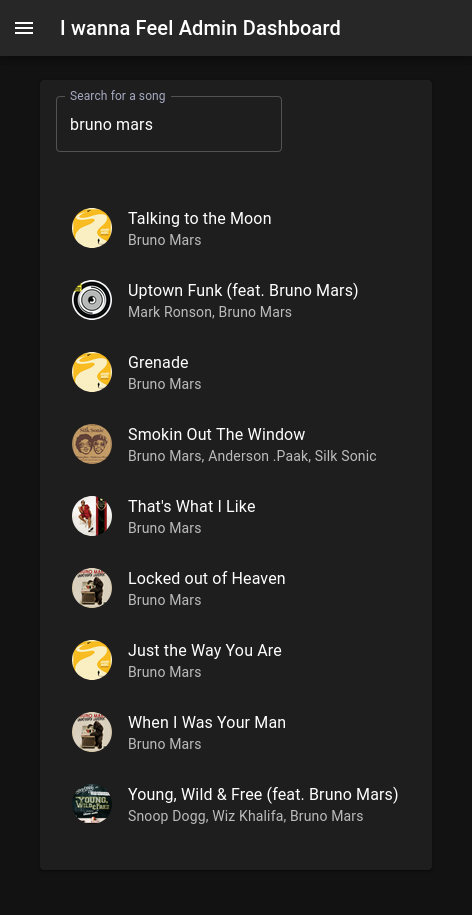
\includegraphics[scale=0.6]{imgs/mobileui2.png}
\caption{Song Search}
\label{fig: mobileUI_2}
\end{figure}

\begin{figure}[H]
\centering
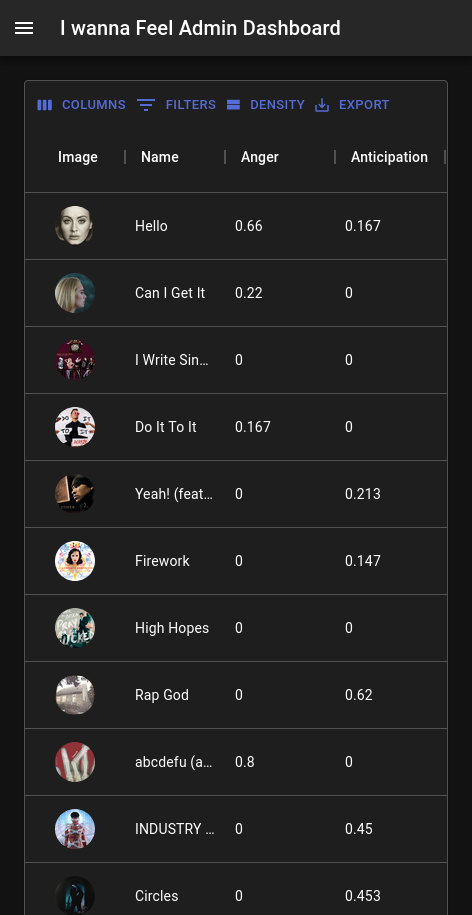
\includegraphics[scale=0.6]{imgs/mobileui3.png}
\caption{Database View}

\label{fig: mobileUI_3}
\end{figure}


\section{User Interface}
\subsection{Landing Page}
\begin{figure}[H]
\centering
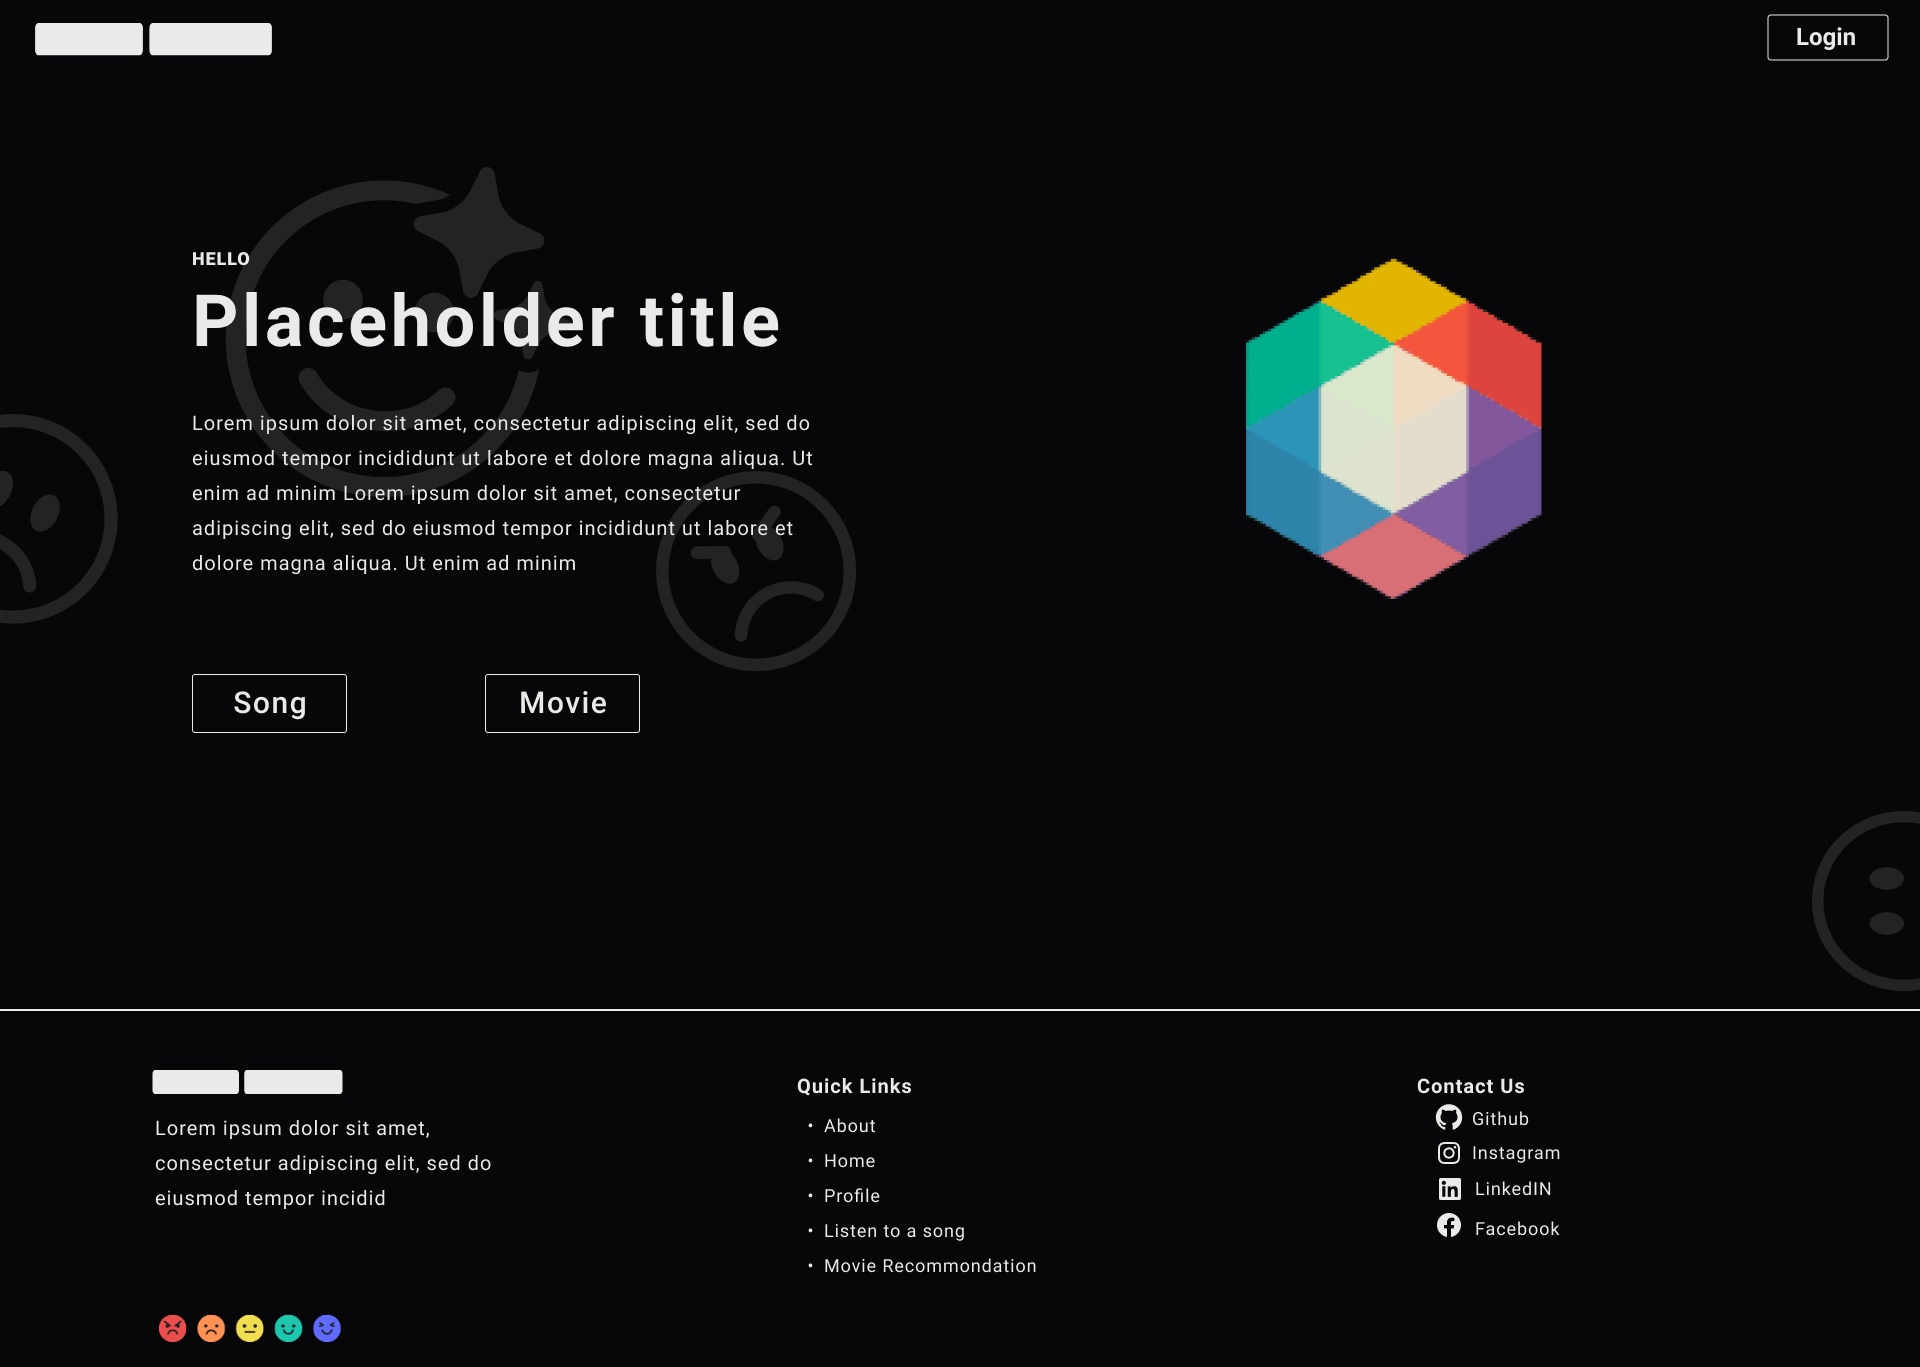
\includegraphics[width=\textwidth]{imgs/ui1.png}
\caption{Landing Page}
\label{fig: ui1}
\end{figure}

This is the home page, here there are 2 primary actions available which directs the user to the song search page or movie search page. The user can also choose to login from this page, but that is available on all pages as well.


\subsection{Emotion Input Pages}
\begin{figure}[H]
\centering
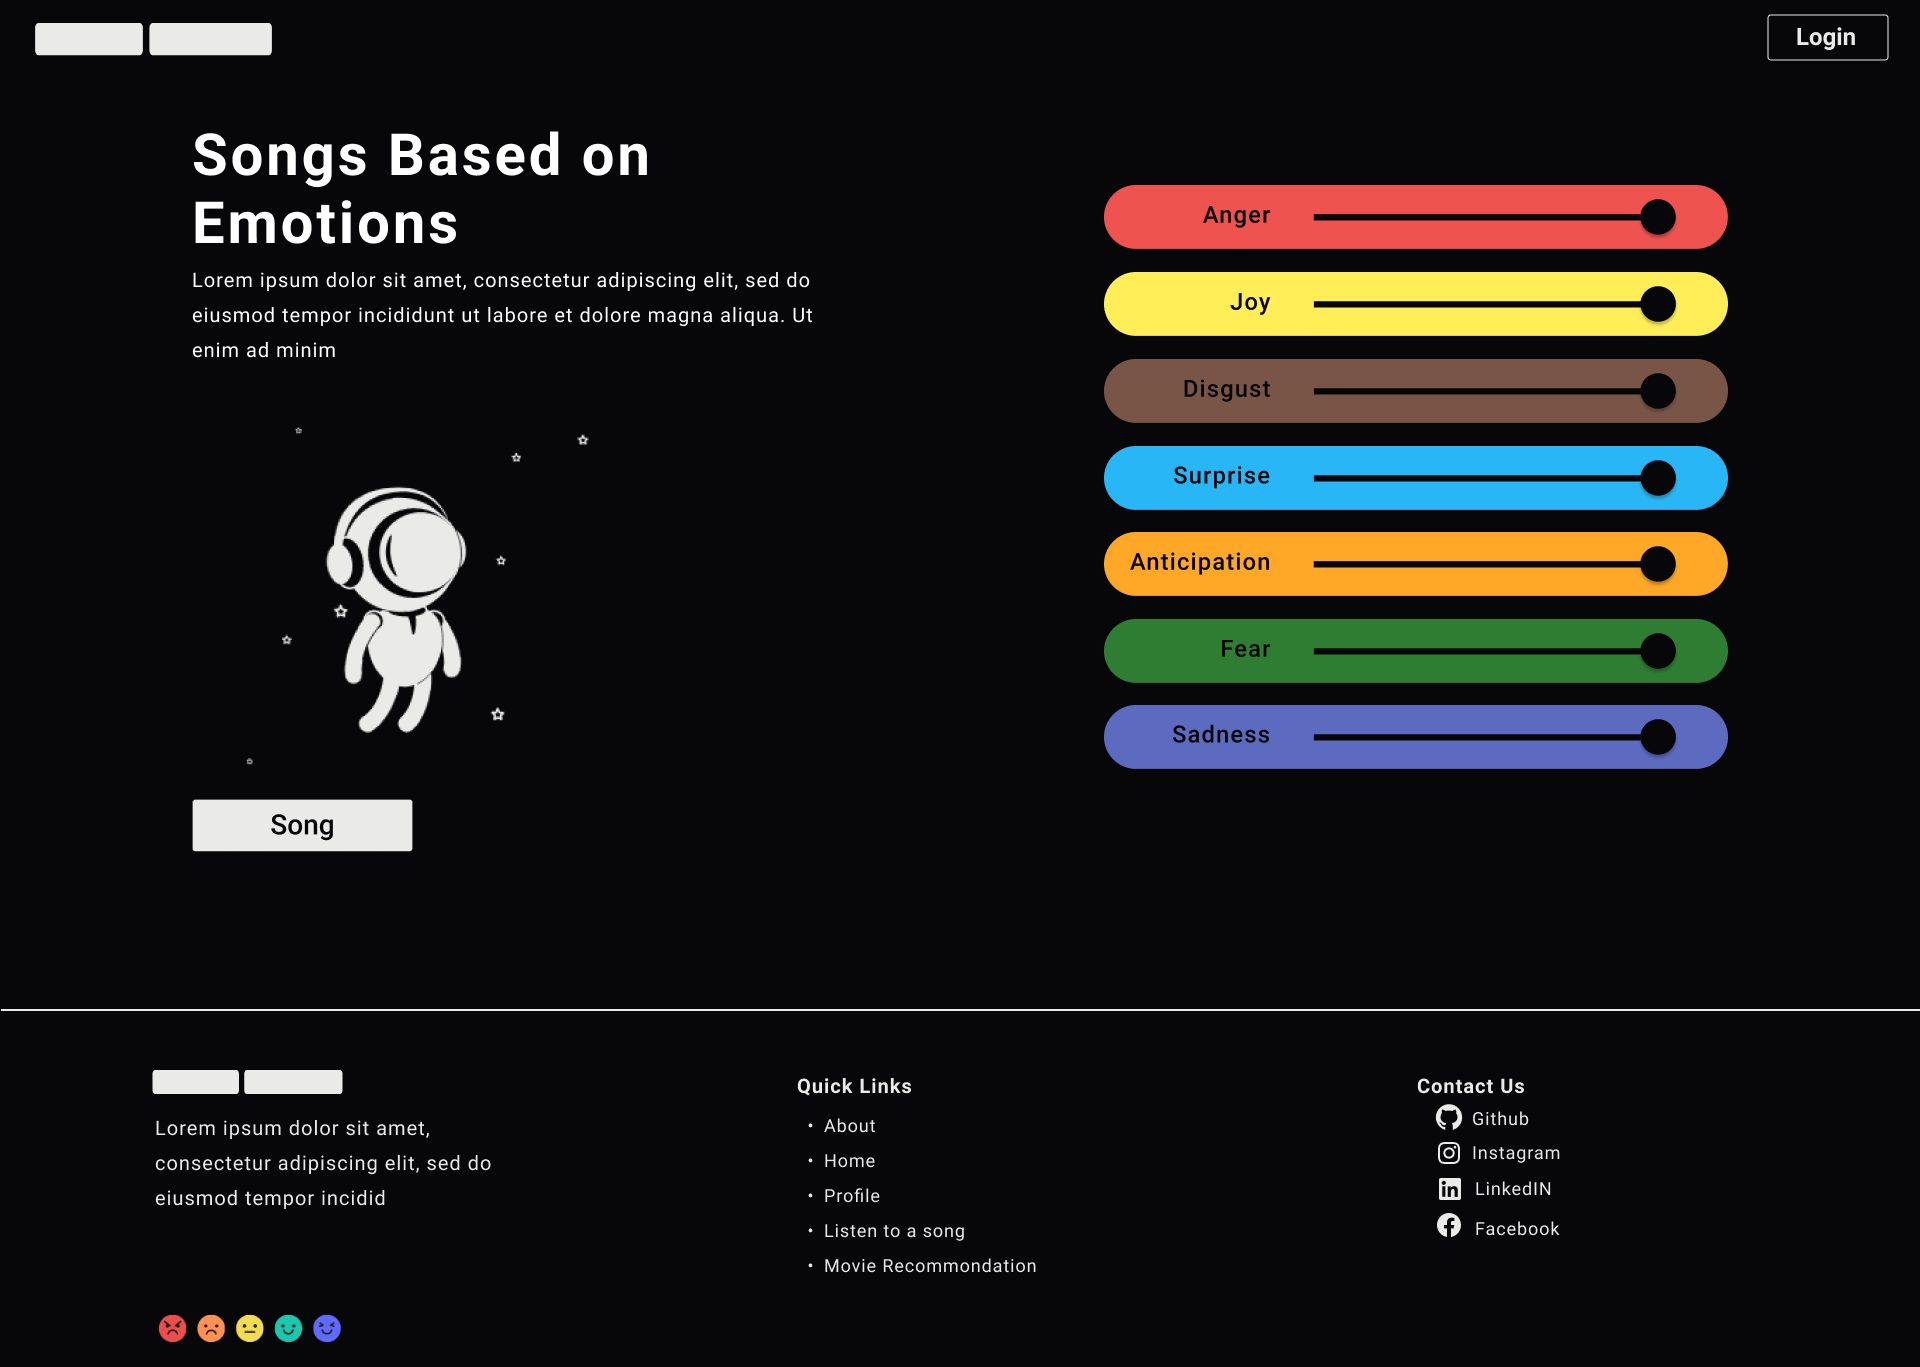
\includegraphics[width=\textwidth]{imgs/ui2.png}
\caption{Song Emotion Input Page}
\label{fig: ui2}
\end{figure}

\begin{figure}[H]
\centering
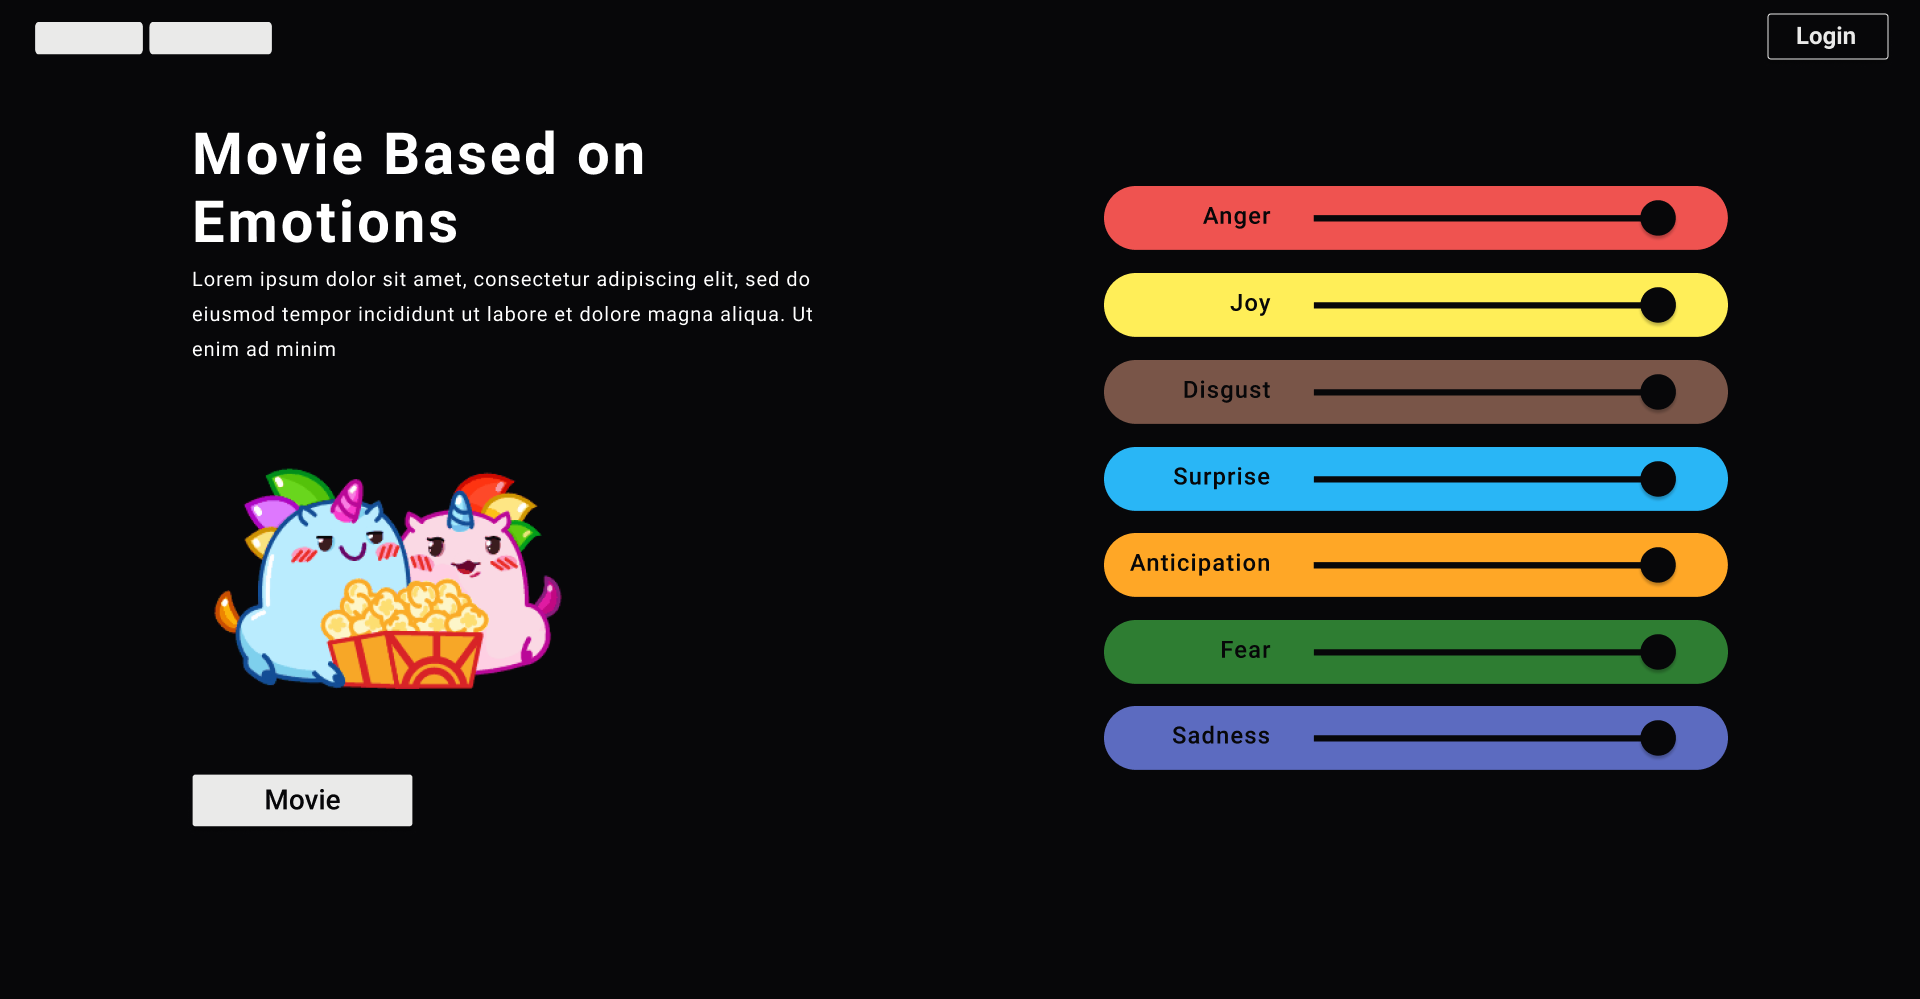
\includegraphics[width=\textwidth]{imgs/ui3.png}
\caption{Movie Emotion Input Page}
\label{fig: ui3}
\end{figure}

These are the emotion input pages, Figure \ref{fig: ui2} for songs and figure \ref{fig: ui3} for movies. Later, we plan to adjust the emotions for songs as we build our dataset. There are various sliders for the different available emotions.

\subsection{Recommendation Pages}
\begin{figure}[H]
\centering
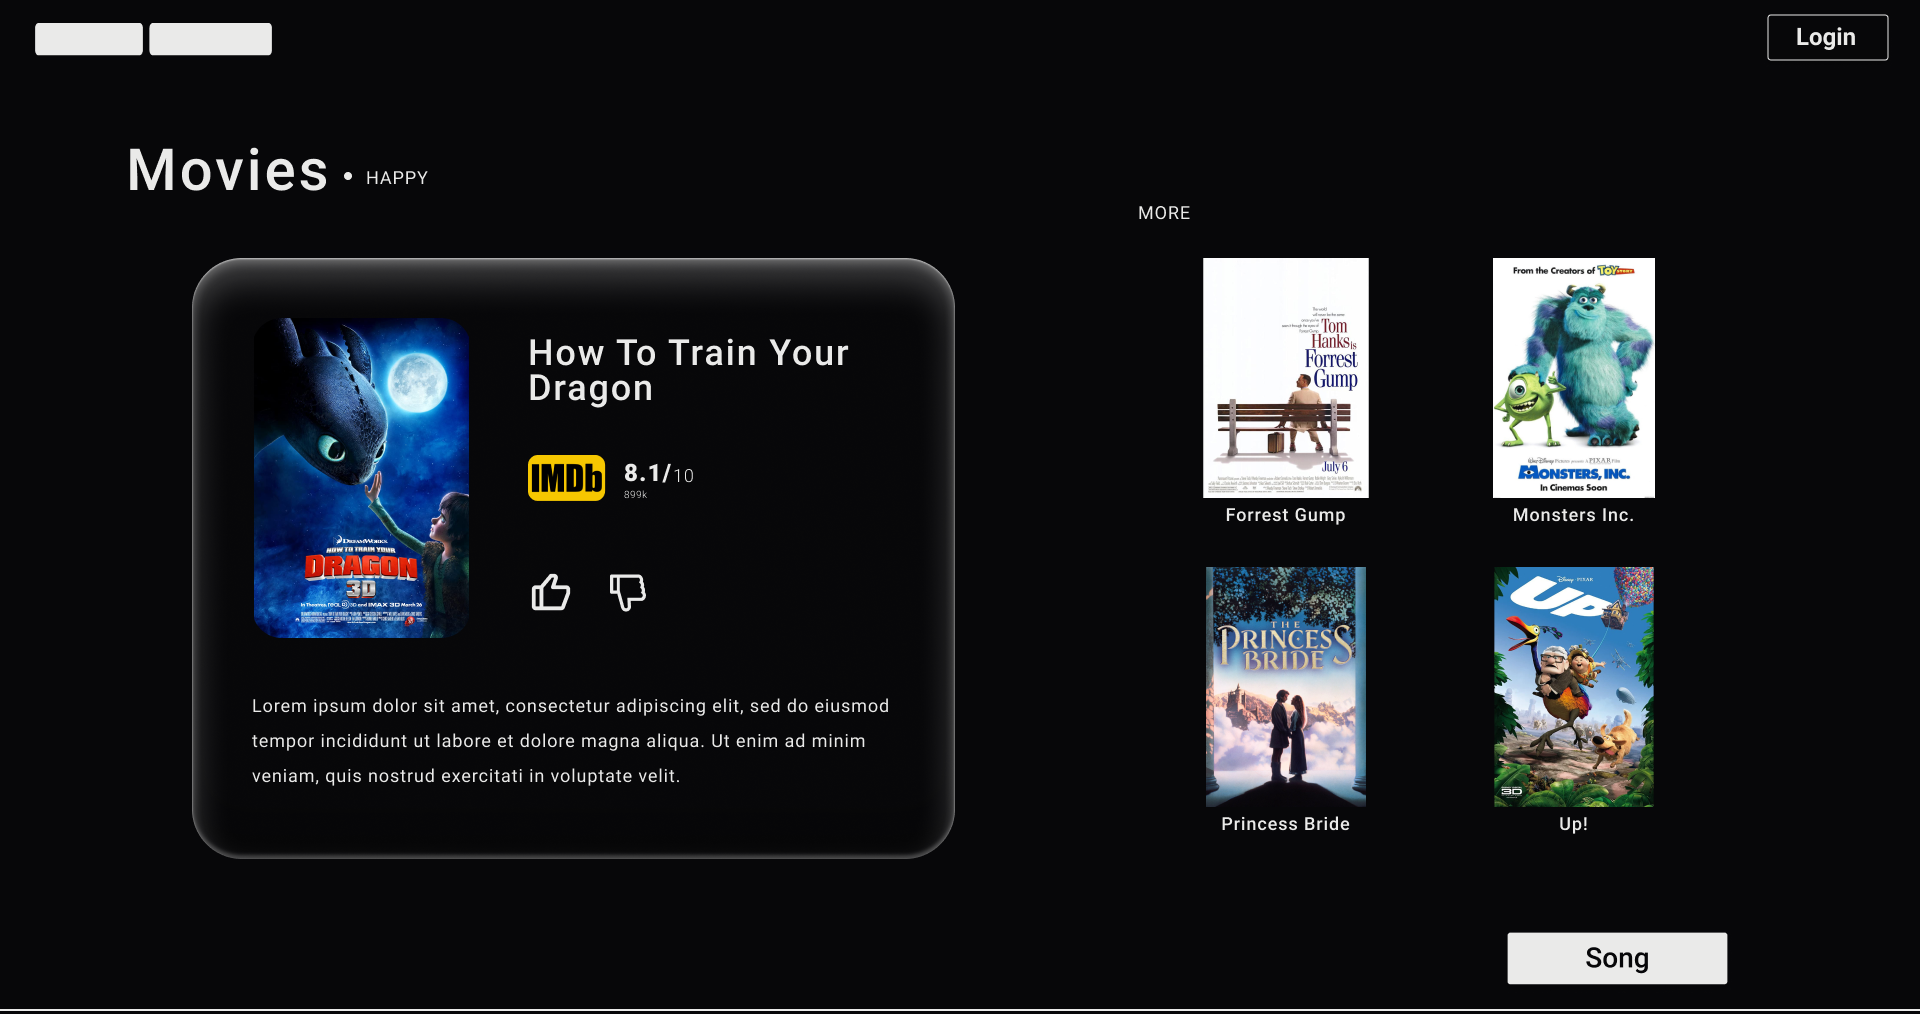
\includegraphics[width=\textwidth]{imgs/ui4.png}
\caption{Movie Suggestion Page}
\label{fig: ui4}
\end{figure}

\begin{figure}[H]
\centering
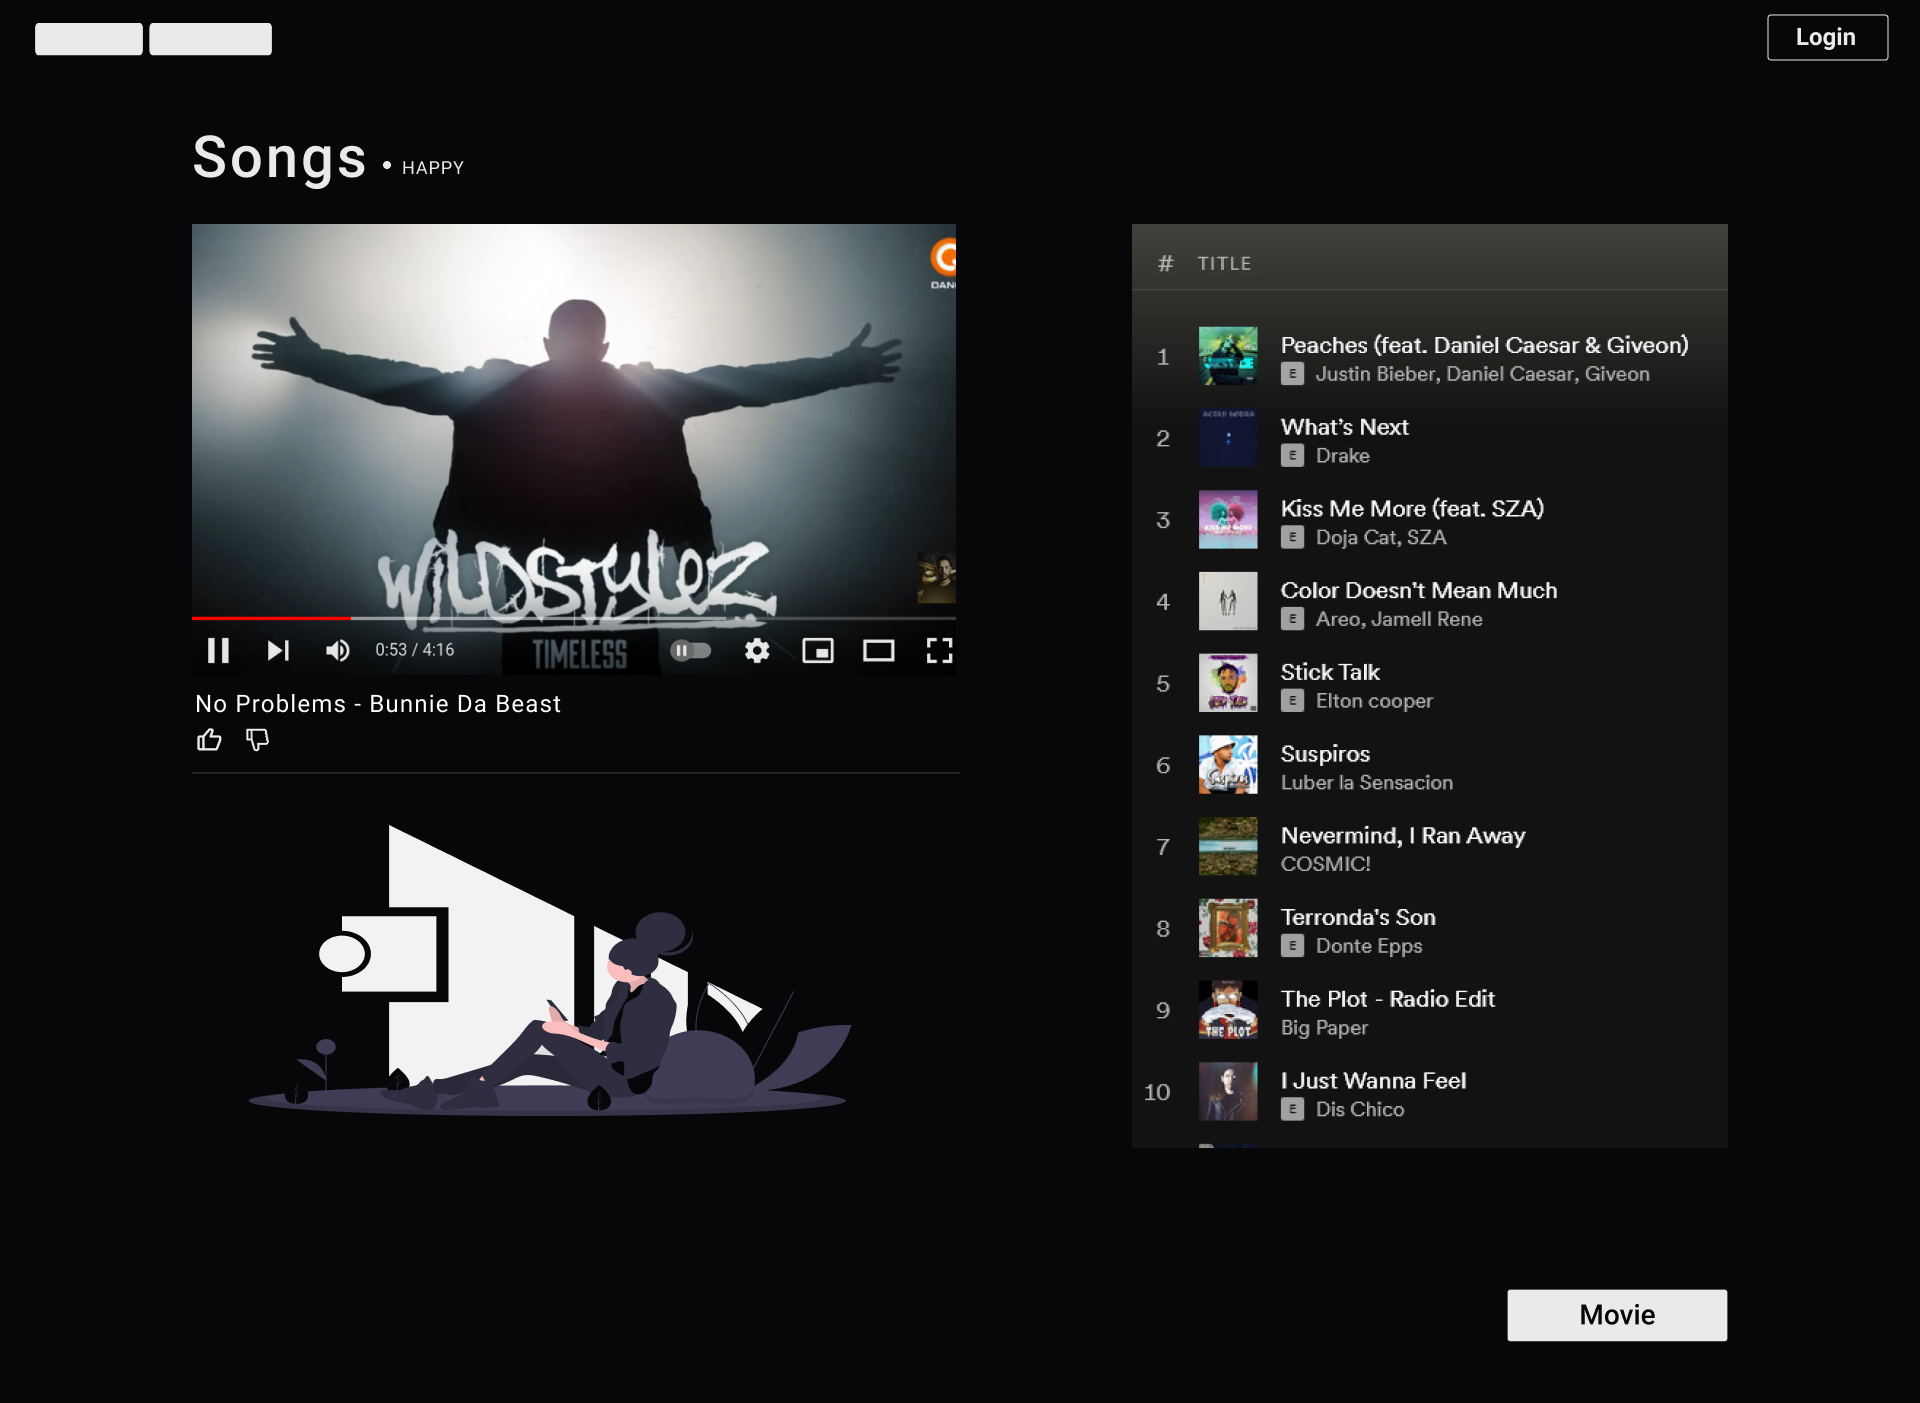
\includegraphics[width=\textwidth]{imgs/ui5.png}
\caption{Song Suggestion Page}
\label{fig: ui5}
\end{figure}
On these pages the user is recommended content based on the emotions inputted from the previous screen. The user is recommended the content in the form of a list, where they can click on it to see more info about it.For songs, we can show an embedded YouTube video. For movies, we can provide a link to IMDB / the content on an OTT platform like Amazon Prime / Netflix.

\subsection{Login Page}
\begin{figure}[H]
\centering
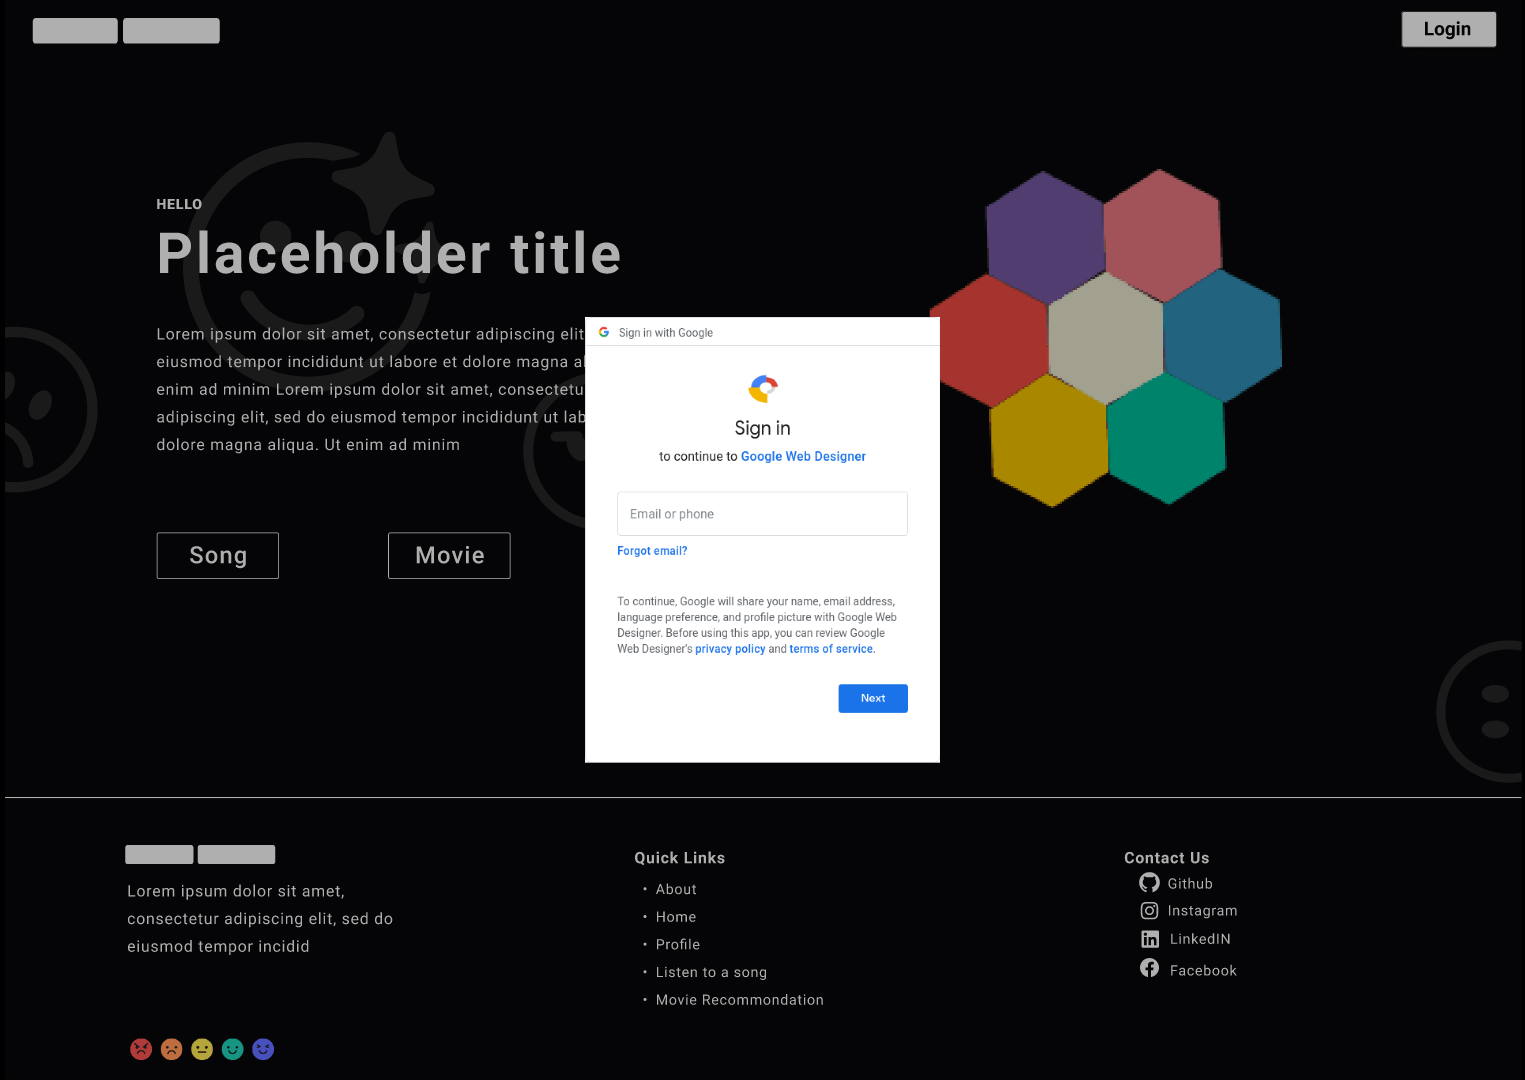
\includegraphics[width=\textwidth]{imgs/ui6.png}
\caption{Login Page}
\label{fig: ui6}
\end{figure}
The login will use Auth0 and will be available across all pages. It will appear as a popup and will provide a one-click login experience. The user will select from a list of services for authentication like Google, Github etc.

